\documentclass{article}
\usepackage{tikz}
\def\mkPascal#1{
  \begin{tikzpicture} 
    \def\dx{20pt}
    \def\dy{30pt}
    \newcounter{i}
    \stepcounter{i}
    \node (\arabic{i}) at (0,0) {1};
    \foreach [count=\i] \x in {2,...,#1}{
      \pgfmathsetmacro{\lox}{\x-1}%
      \pgfmathsetmacro{\loxt}{\x-3}%
      \foreach [count=\j] \xx in {-\lox,-\loxt,...,\lox}{
        \pgfmathsetmacro{\jj}{\j-1}%
        \stepcounter{i}
        \pgfmathsetmacro{\lbl}{\lox!/(\jj!*(\lox-\jj)!)}
        \node  (\arabic{i}) at (\xx*\dx, -\lox*\dy) {\pgfmathint{\lbl}\pgfmathresult};
      }
    }
    \newcounter{z}
    \newcounter{xn}
    \newcounter{xnn}
    \pgfmathsetmacro{\maxx}{#1 - 1}
    \foreach \x in {1,...,\maxx}{
      \foreach \xx in {1,...,\x}{
        \stepcounter{z}
        \setcounter{xn}{\arabic{z}}
        \addtocounter{xn}{\x}
        \setcounter{xnn}{\arabic{xn}}
        \stepcounter{xnn}
          \draw [->] (\arabic{z}) -- (\arabic{xn});
          \draw [->] (\arabic{z}) -- (\arabic{xnn});
      }
    }
  \end{tikzpicture}
}
\usepackage{amssymb}
\usepackage{amsmath}
\usepackage{blindtext}
\usepackage{multirow}
\usepackage{graphicx}
\usepackage{cancel}
\usepackage{color}
% load the geometry package
\usepackage[letterpaper,
            left=1cm,right=1cm,
            top=2cm,bottom=4cm]{geometry}         
\title{Math 251: Problem Set I.}
\author{Jason Krivo Flores}
\date{\today} 
\begin {document}
\maketitle{}
%
\begin{enumerate}
 \item Consider the piecewise defined function defined below:\\
\[
  f(x) = \left\{ 
  \begin{array}{l l}
    \frac{ sin(\theta)}{\theta}, \quad &  \theta \neq 0\\
    \\
      \frac{1}{2},  \quad &  \theta= 0\\
  \end{array} \right. \\
\]
\\
The domain of the function is $(-\infty, \infty)$
$f(x)$ is sinusoidal and continuous for all values $\neq 0$.\\ When $\theta = 0$ The function exhibits a ``Jump'' discontinuity and returns a fixed value of $y = \frac{1}{2}$.\\
A graph of this function (figure 1.) shows these properties. Notice also that as $x \to 0$ the $ \lim f(x) $ approaches 1.\\
(We are not proving this result here but merely showing graphically its tendency)\\
\\(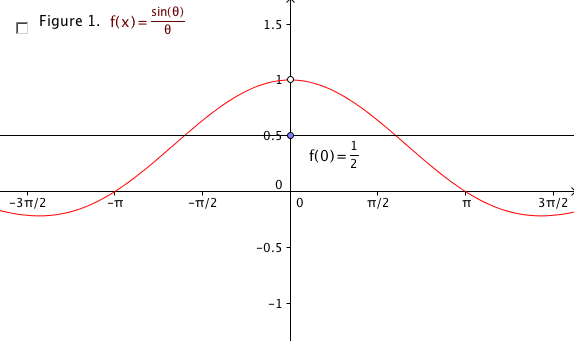
\includegraphics[scale=0.5]{singraph}\\
There are several other interesting features to note: Although this function approaches a general limit of 1 as $\theta_\to 0$ from both the left and the right, the actual value of $f(0) = \frac{1}{2}$.\\
\\
\\As x approaches infinity $f (x) \to 0$ (figure 2.)\\
%
{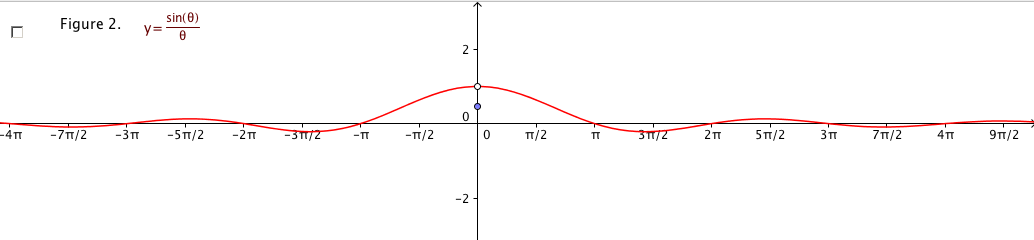
\includegraphics[scale=0.5]{longview}}\\

\pagebreak
Examine the function below:\\
\\
\fbox{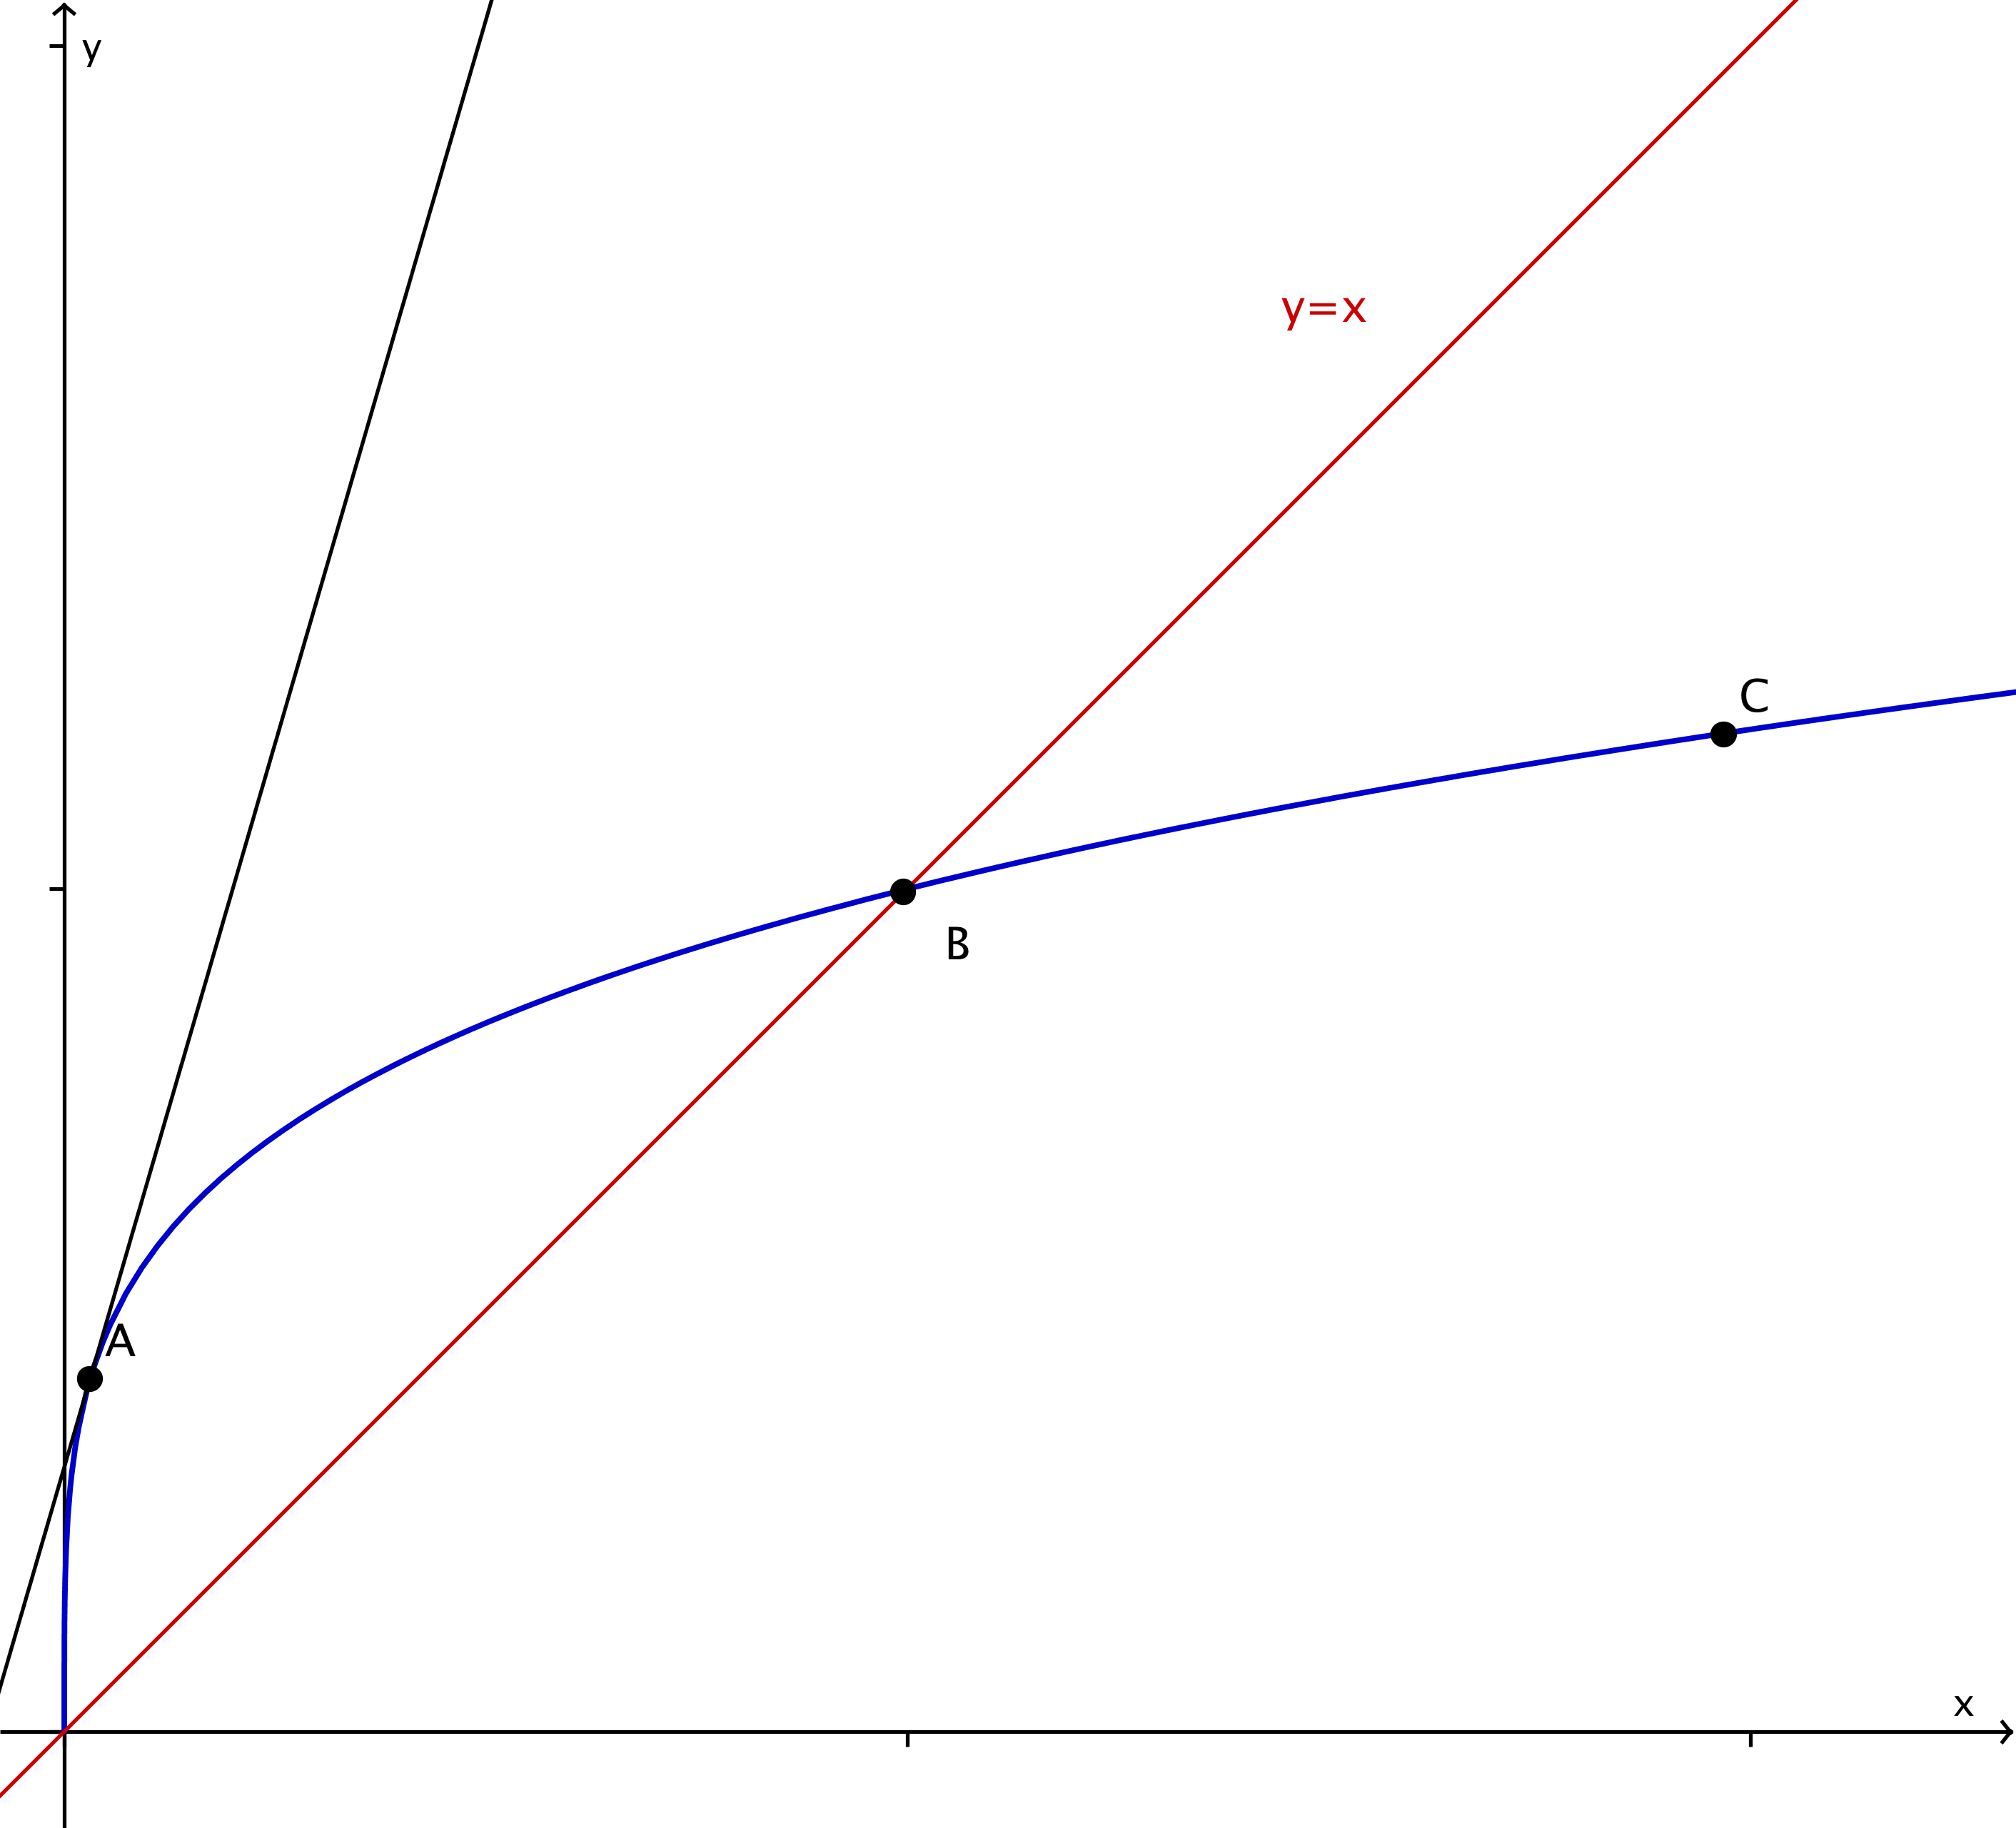
\includegraphics[scale=0.4]{loggy}}\\
%
\\Given only the information contained in the graph, is it possible to arrange the following quantities in increasing order? 
%
\begin{itemize}
%
	\item The slope of the tangent line to the graph at point A
	\item The slope of the tangent line to the graph at point B
	\item The slope of the tangent line to the graph at point C
	\item The slope of the line that contains points A and B
	\item The number 0
	\item The number 1
%	
\end{itemize}
The function appears to be of the form$f(x)= \sqrt{x}$ but no explicit formula is given nor are the axes enumerated. The coordinates of the points (A,B, and C) have also been withheld.  \\

Before we despair, let's take inventory of what we \emph have been given: The $x$ and$ y$ axes, and the line {\color{red}$y = x$} and that is all the information we need to derive our slopes. \\

Recall the slope of a line is calculated by the change in $y$ of a line over the change in $x$ also known as, $\frac{\text \bfseries RISE}{\text \bfseries RUN}$.
A line with the equation $y=x$ therefore has a slope of 1 as will any line parallel to it.\\ The x axis and lines parallel have a slope of zero. From this we can infer that lines which fall between the x axis and the line $y=x$ have slopes that are proper fractions (the line rises fewer than one unit per unit distance travelled the closer it gets to s slope of 0). Conversely, lines that fall between line $y=x$ and the $y$ axis are improper fractions that increase in slope the close they parallel the $y$ axis (though lines {\emph exactly} parallel to the $y$ axis have an undefined slope. \\

Now lets arrange our items in increasing order, first 0 is the smallest as we have no negative quantities, next we need to find the lines most closely parallel to the $x$ axis.

\pagebreak

View figure 2.3.\\
\fbox { 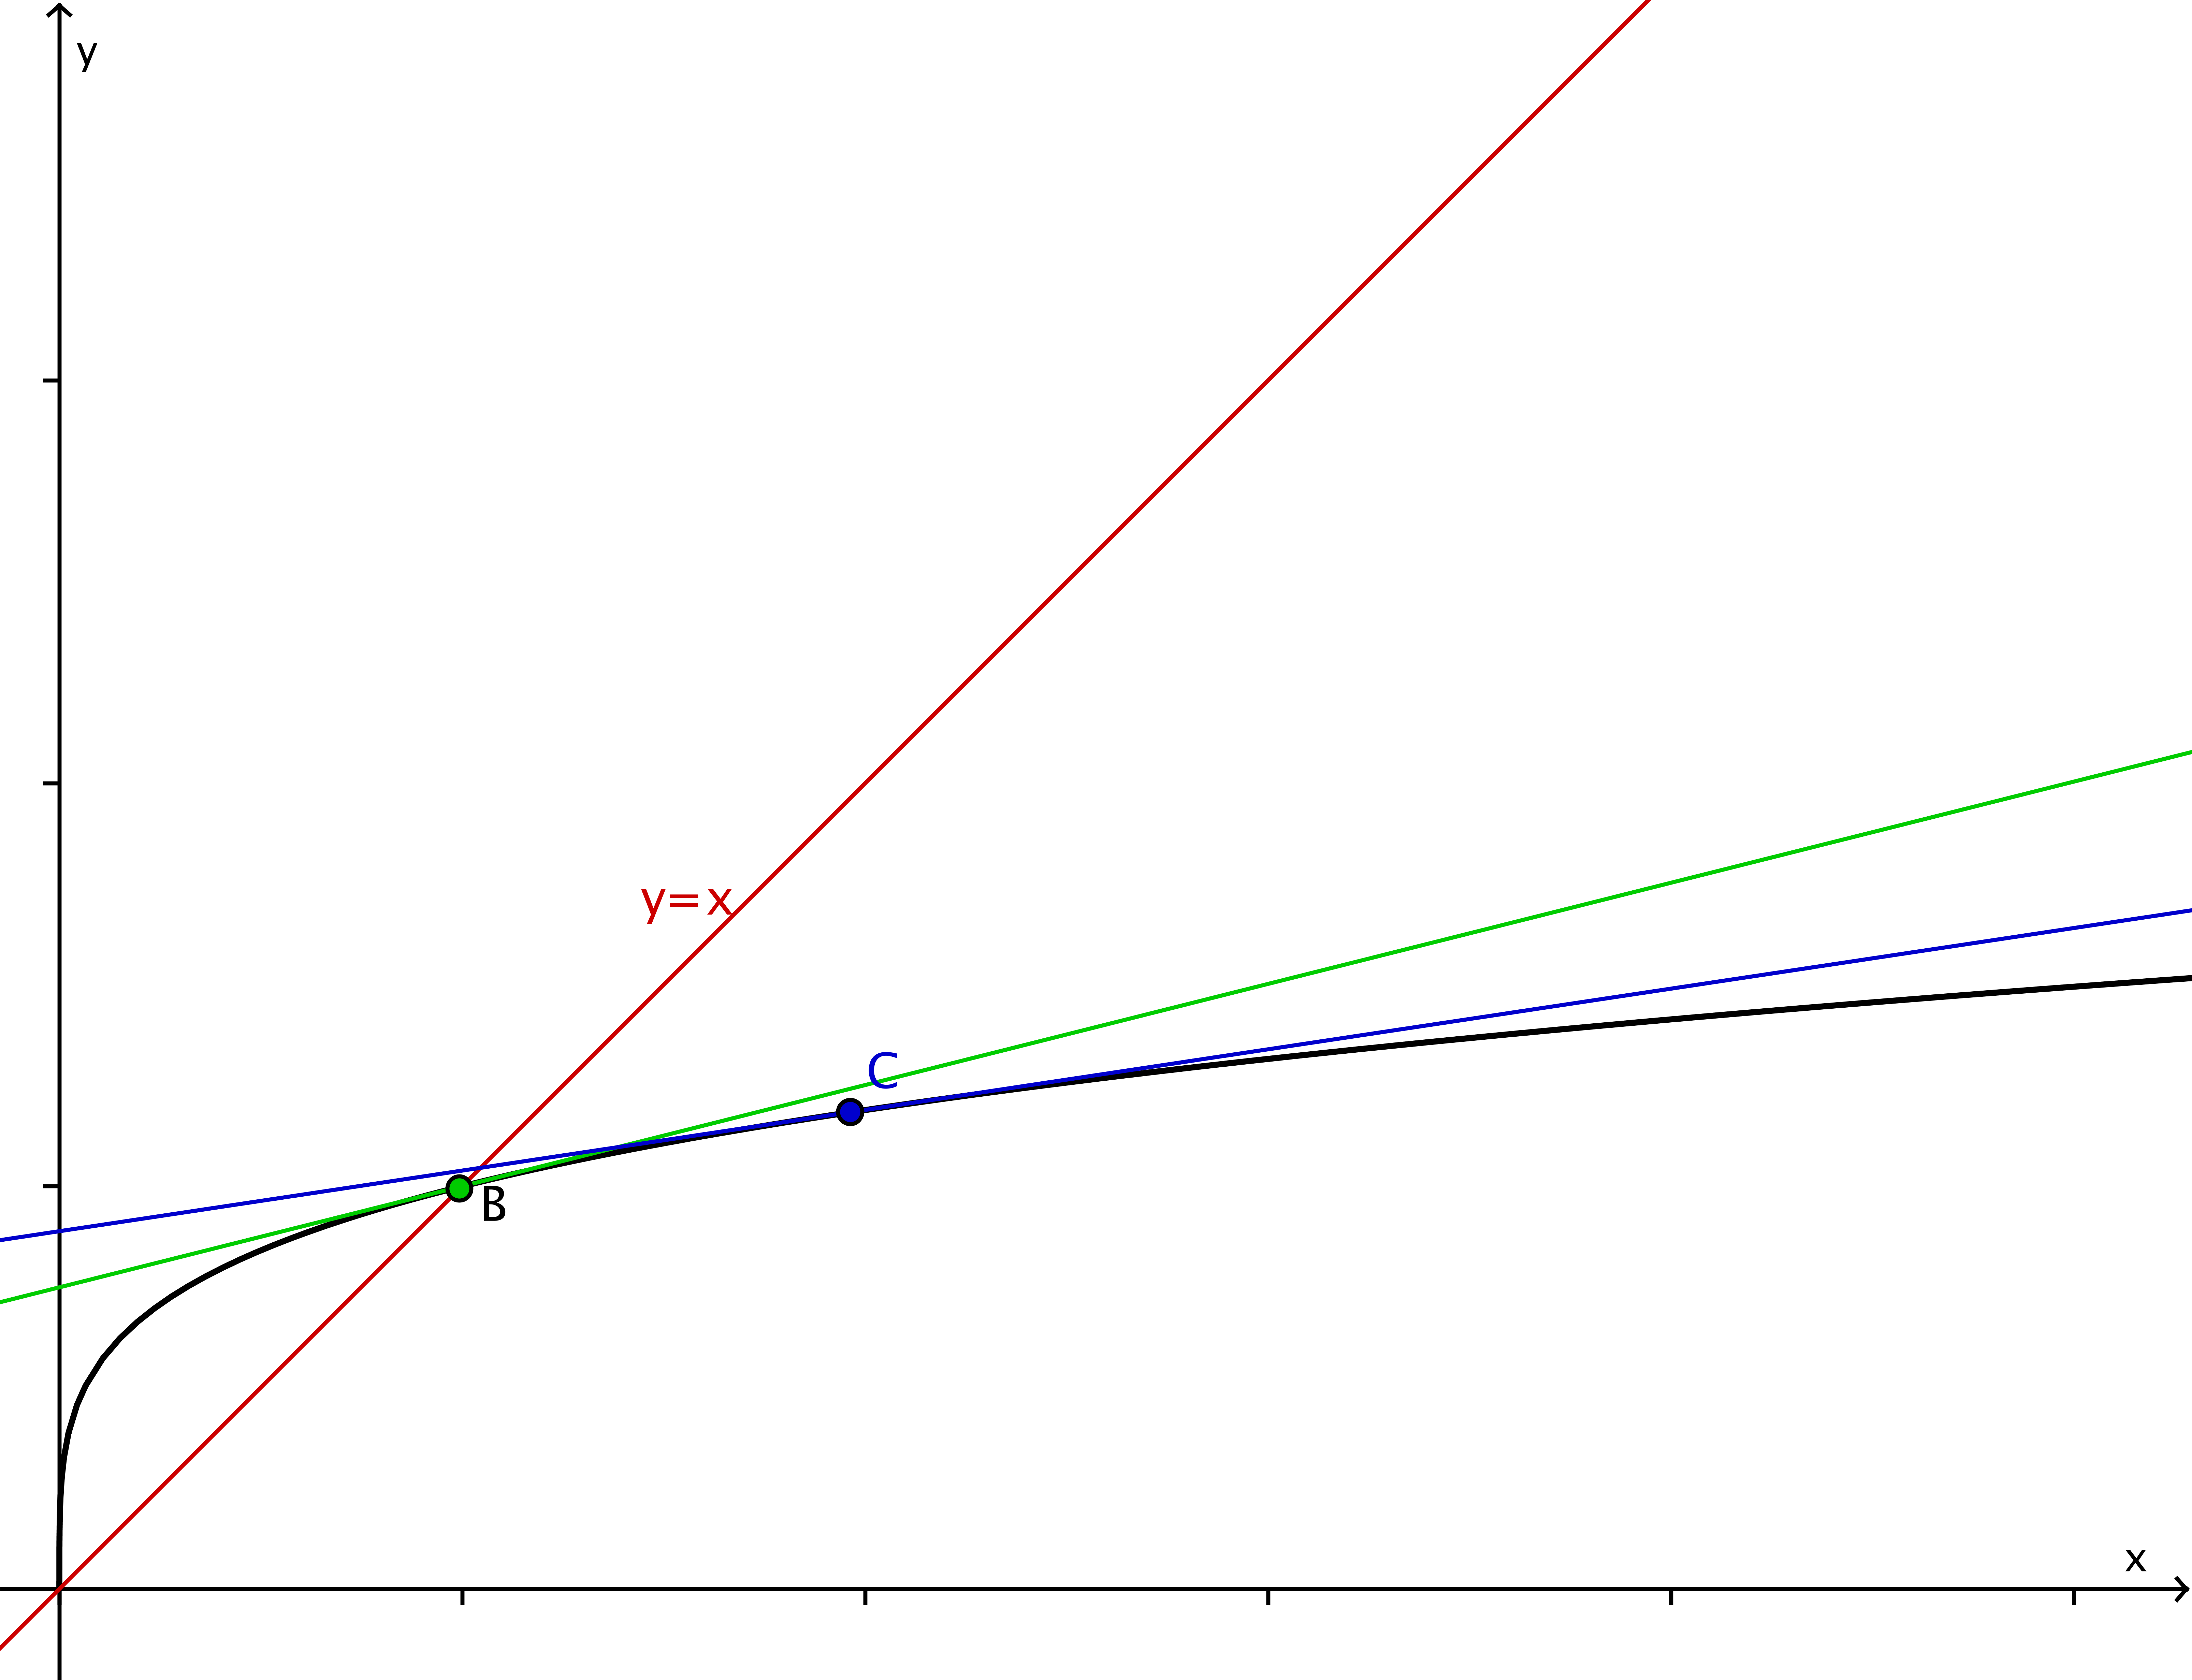
\includegraphics [scale= 0.19] {AB} } \\ 

Recall, a tangent line to a curve is a line that touches it at only one point and is its best straight line approximation. I have drawn color coded tangent lines at points { \color{green}{B}} and {\color{blue}{C}} on the graph 2.3.  Notice both lines lie between {\color{red} $y=x$} and thus have a slope $< 1$. The tangent line to point {\color{blue}{C}} most closely parallels the x axis and therefore is our second smallest quantity followed by the tangent line to { \color{green}{B}}. \\

We can assess our final quantities with figure 2.3\\

\fbox{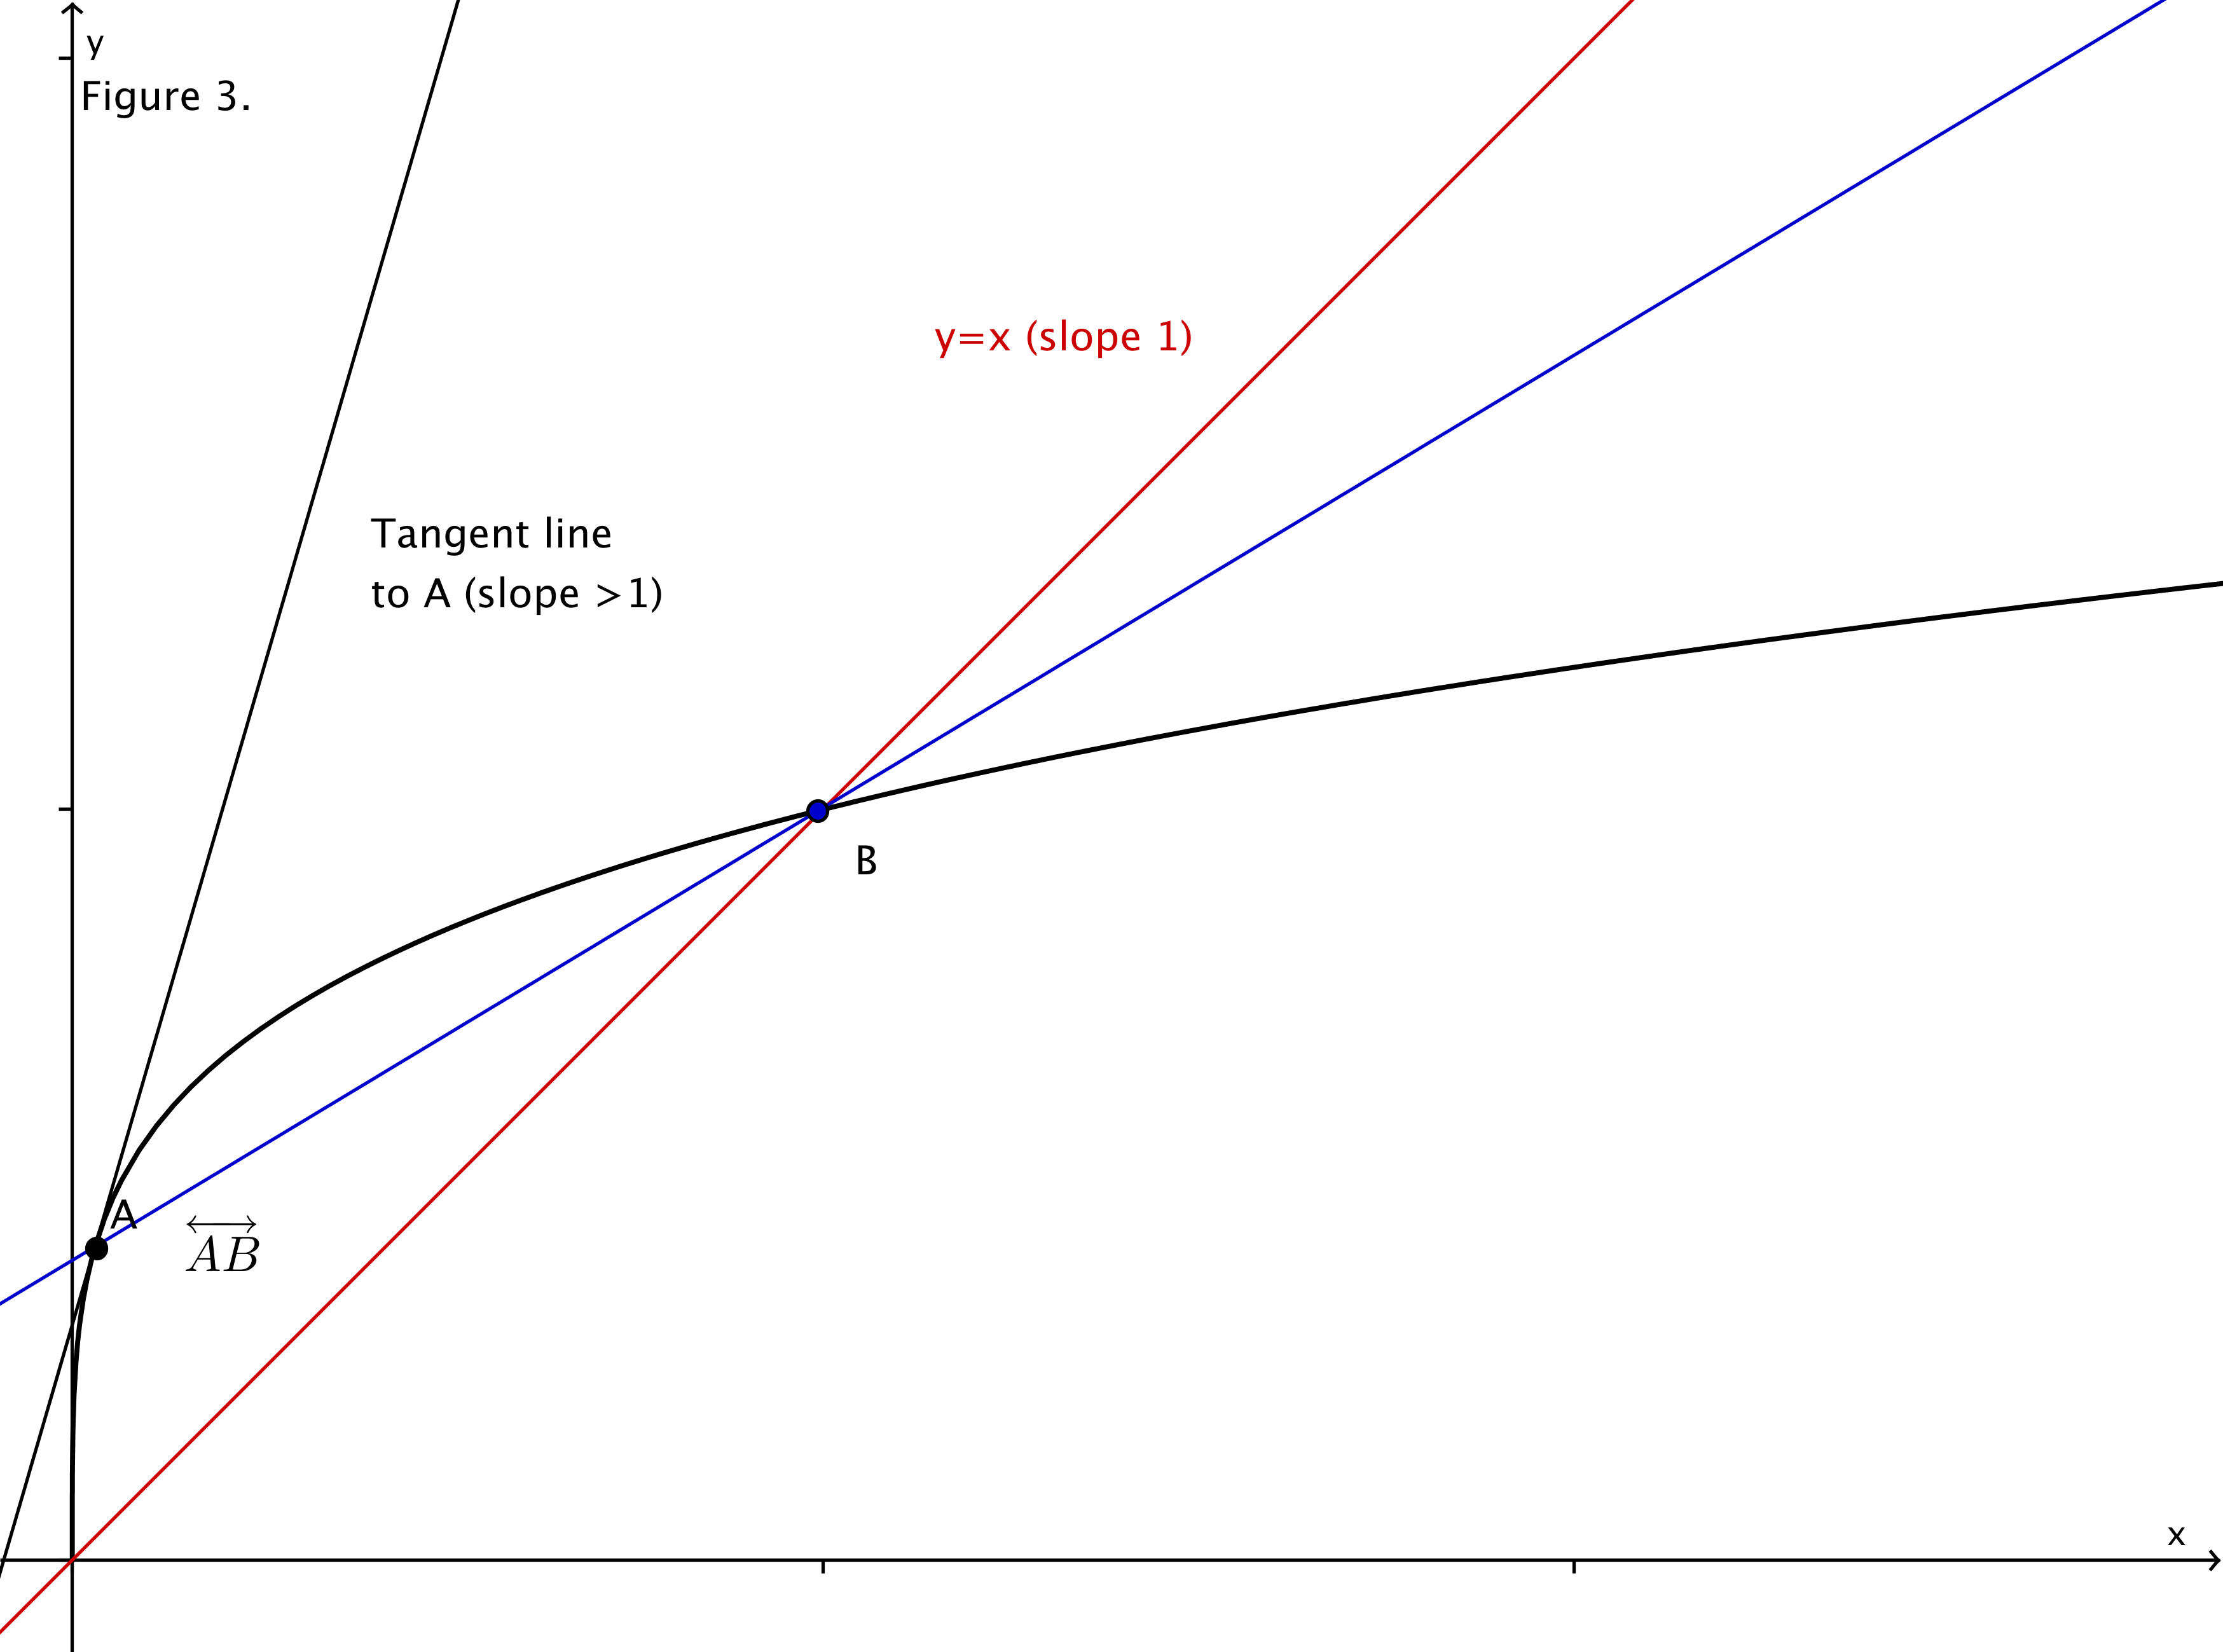
\includegraphics[scale= 0.35]{slopey}}\\ 
  
The tangent line to point A is the closest to the $y$ axis and our only quantity $ > 1$, as the line $\overleftrightarrow{AB}$ also falls between $y=x$ and the $x$ axis but is nearest to the line $y=x$. \\

{\bfseries We now can arrange our quantities in increasing order: 0, TanC, TanB, $\overleftrightarrow{AB}$, 1, and TanA.}
 
\end{enumerate}



\begin{itemize}
\item The Figure below is known as Pascal's Triangle, it has many interesting and useful properties: \\
The edges are all the number 1. The diagonals beginning with the second row from the top are the counting numbers 1,2,3,4 . . .  \\
 
The horizontal rows are powers of 11( $ 11^0=1, 11^1= 11, 11^2=121, 11^3=1331$, etc.) and the whole array is left/right symmetric. \\ 

The top row that is the single digit ``1'' is known as the ``zeroth'' row. The first row is 1,2, and so forth.
%
\end{itemize}
%
\mkPascal{8} \\

{\center Watch what happens when we expand the following expressions:}
 
\begin{align*}
  (a + b)^0 &= a + b\\
  (a + b)^2 &= a^2 + 2ab + b^2\\
  (a + b)^3 &= a^3 + 3a^2b + 3ab^2 + b^3\\
  (a + b)^4 &= a^4 + 4a^3 b + 6a^2b^2 + 4ab^3 + b^4\\
  (a + b)^5 &= a^5 + 5a^4 b + 10a^3 b^2 + 10a^2 b^3 + 5ab^4+b^5
\end{align*} 
 
The horizontal rows of pascals triangle correspond to the coefficients of our binomial expansions. $(a+b)^0$ corresponding to the zeroth row has a coefficient of ``1''.  $(a+b)^2$`s coefficients are 1,2,1 the same as its expansion $ a^2+2ab+b^2$.
  
\end {document}